\documentclass{book}
\usepackage{graphicx}
\usepackage[english]{babel}
\usepackage{amsthm}
\usepackage{amsmath}
\usepackage{amssymb}
\usepackage{amsfonts}
\usepackage{physics}
\usepackage{tikz}
\usepackage[a4paper, margin=1in]{geometry}
\geometry{a4paper, margin=1in}
\usepackage{xcolor}
\graphicspath{ {./images/} }
\usepackage{svg}
\usepackage{bm}
\usetikzlibrary{patterns, patterns.meta}
\usetikzlibrary{angles, quotes}
\usetikzlibrary{backgrounds,matrix,patterns}
\usetikzlibrary{patterns.meta, fit}
\usepackage{mathtools}
\usepackage{pgfplots}
\usepackage{subfigure}
\usepackage{subcaption}
\usepackage[affil-it]{authblk}
\usepackage{xcolor}
\usepackage{array} % for defining a new column type
\usepackage{varwidth} %for the varwidth minipage environment
\usepackage{appendix}

\usetikzlibrary{decorations.pathmorphing,patterns}
\renewcommand{\cleardoublepage}{\clearpage}
\pgfplotsset{compat=1.18}
\newtheorem*{definition}{Definition}

\title{Vibrations and Waves}
\author{Dominik Szablonski}

\begin{document}

\maketitle

\tableofcontents

\chapter{Simple Harmonic Motion}
\begin{definition}[Simple Harmonic Motion]
    The oscillation of a quantity about some equilibrium point due to being trapped in a potential well.
\end{definition}
\begin{figure}[h]
\begin{center}
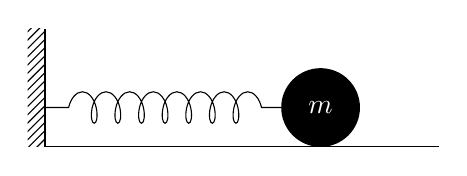
\begin{tikzpicture}
    \draw[thick] (0,0) -- (0,1.5);
    \fill[pattern=north east lines] (0,0) rectangle (-0.22,1.5);
    \draw
        [
            decoration={
                coil,
                segment length = 3mm,
                amplitude = 2mm,
                aspect = 0.5,
                post length = 2mm,
                pre length = 3mm},
    decorate] (0,0.5) -- (3,0.5);
    \fill[black] (3.5,0.5) circle (0.5);
    \draw (0,0) -- (5,0);
    \node at (3.5,0.5) {\textcolor{white}{$m$}};
\end{tikzpicture}
\end{center}
\caption{A mass resting on a friction-less surface attached to a spring.}
    \label{fig:enter-label}
\end{figure}

\noindent
Let us first consider a mass extending a spring while on a friction-less surface. We know by Hooke's law (for small displacements),
\begin{equation*}
    F = -kx.
\end{equation*}
We can apply Newton's second law to get,
\begin{equation}
    m\Ddot{x} = -k x,
\end{equation}
which we can rewrite,
\begin{equation}\label{differential}
    \Ddot{x} = -\omega^2x
\end{equation}
where,
\begin{equation}
    \omega^2 = \frac{k}{m}.
\end{equation}
Equation \eqref{differential} has a general solution,
\begin{equation}\label{springsolution}
    x(t) = A\cos(\omega t + \phi)
\end{equation}
where $A$ is the amplitude of the motion and $\phi$ is the phase.
\section{Energy in SHM}
We know that generally,
\begin{equation}
    E = K + U.
\end{equation}
For a spring, this is,
\begin{equation}\label{energy}
    E = \frac{1}{2}mv^2 + \frac{1}{2}kx^2,
\end{equation}
which, when substituting equation \eqref{springsolution},  equation \eqref{energy} reduces to,
\begin{equation}
    E = \frac{1}{2}kA^2.
\end{equation}
Thus, we can conclude that $E \propto A^2$. Therefore, the more we initially extend the spring, the more potential energy we can store in it. 
\section{SHM In All Systems}
Provided that the amplitude of oscillation is small, a system will exhibit simple harmonic motion. This is because small displacements from a system's stable equilibrium resemble a parabola. We can prove this by considering the Maclaurin expansion of the potential energy,
\begin{equation*}
    U(x) = U_0 + x\left( \dv{U}{x} \right)_{x=0} + \frac{1}{2}x^2\left(\dv[2]{U}{x}\right)_{x=0}.
\end{equation*}
$U_0$ is an additive constant, so can be set to 0. Since the system is at equilibrium at $x=0$, $\left(\dv{U}{x}\right)_{x=0}$ can also be set to 0. Thus, the potential energy is given by,
\begin{equation}
    U(x) \approx \frac{1}{2}x^2\left(\dv[2]{U}{x}\right)_{x=0}.
\end{equation}
Force is negative gradient of potential, so,
\begin{equation}
    F = -x\left(\dv[2]{U}{x}\right)_{x=0},
\end{equation}
which is the form of the equation of SHM.
\subsection{Examples of Other Forms of SHM}
\subsubsection{Pendulum}
\begin{figure}[h]
        \centering
        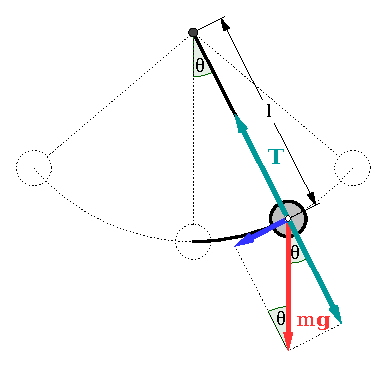
\includegraphics[width=200pt]{pendulum.pdf}
        \caption{Diagram of a pendulum.}
        \label{fig:pendulum}
\end{figure}
\noindent
By using the small angle approximation, we are able to write the equation of motion of the pendulum,
\begin{equation}
    \Ddot{\theta} = -\frac{g}{l}\theta.
\end{equation}
for which the energy will be equal to,
\begin{equation}
    \begin{split}
        E & = \frac{1}{2}mv^2 + \frac{1}{2}\frac{mgx^2}{l} \\
        & = \frac{1}{2}\frac{mgA^2}{l}
    \end{split}
\end{equation}
where $x$ is the horizontal distance from the equilibrium that the pendulum moves.
\subsubsection{LC Circuit}
\begin{figure}[h]
    \centering
    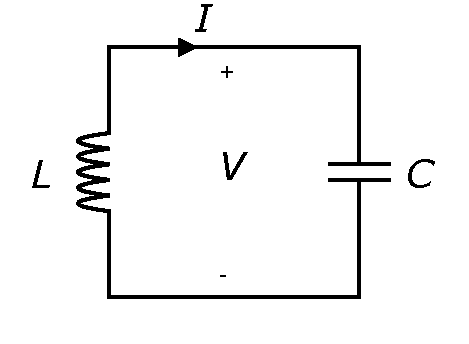
\includegraphics[width=150pt]{LC.pdf}
    \caption{Diagram of the LC circuit we are considering.}
    \label{fig:LC}
\end{figure}
Figure \ref{fig:LC} represents an inducer circuit charging a capacitor. We should expect the current to oscillate between the plates of the conductor. We can begin by understanding that the total charge in the system is equal to 0, which we can write as,
\begin{equation}
    L\dv{I}{t} + \frac{q}{C} = 0.
\end{equation}
Differentiating this, we get the expression,
\begin{equation}
    \dv[2]{I}{t} = -\frac{1}{LC}I,
\end{equation}
which is an equation of SHM.
\section{General Form of SHM}
From the examples, it is clear that any oscillating quantity can exhibit SHM. We can define the general differential equation as,
\begin{equation}
    \alpha \dv[2]{Z}{t} = -\beta Z.
\end{equation}
whose solution will be,
\begin{equation}
    Z(t) = Z_0 \cos\left(\sqrt{\frac{\beta}{\alpha}}t + \phi\right),
\end{equation}
and whose energy can be written as,
\begin{equation}
    E = \frac{1}{2}\alpha\left(\dv{Z}{t}\right)^2 + \frac{1}{2}\beta Z^2.
\end{equation}
The symbols are defined as follows,
\begin{definition}[$Z$]
    This is the oscillating quantity.
\end{definition}
\begin{definition}[$\alpha$]
    This is a constant representing the inertia of a system (e.g., mass, moment of inertia, etc.).
\end{definition}
\begin{definition}[$\beta$]
    This is a constant representing the restoring force per unit displacement through which the potential energy is stored (i.e., force due to gravity in a pendulum).
\end{definition}
\begin{definition}[$Z_0$]
    The amplitude of the oscillating quantity.
\end{definition}
\subsection{Period Independent of Mass: Proof by Dimensional Analysis}
\chapter{Damped Harmonic Motion}
Most oscillatory motion feels a damping force, such that,
\begin{equation}
    F_D = -bv
\end{equation}
where $b$ is a positive constant. Including this in the equation of motion, we get
\begin{equation}\label{eqdamp}
    \Ddot{x} + \gamma \Dot{x} + \omega_0^2x = 0.
\end{equation}
where $\omega_0$ is the \textbf{undamped natural frequency}, and
\begin{equation}
    \gamma = \frac{b}{m}.
\end{equation}
We should note that the the force being linearly proportional to velocity is only a very good approximation, and works when the velocity of the system is small.
\section{Light Damping}
For light damping, the oscillator retains its oscillatory behaviour but its amplitude decays with time. The solution to equation \eqref{eqdamp} is,
\begin{equation}
    x(t) = Ae^{-\beta t }\cos(\omega t + \phi)
\end{equation}
where,
\begin{equation}
    \beta = \frac{\gamma}{2},
\end{equation}
and
\begin{equation}
    \omega^2 = \omega_0^2 - \frac{\gamma^2}{4}
\end{equation}
which is called the \textbf{damped angular frequency}. A key property of damped harmonic motion is that,
\begin{equation}
    \omega_0^2 > \frac{\gamma^2}{4}.
\end{equation}
\section{Heavy Damping}
In heavy damping, oscillations are suppressed and the system stops moving before it completes any oscillations. In this case, the solution will be in the form,
\begin{equation}
    x(t) = e^{-\beta}f(t)
\end{equation}
where $f(t)$ is an unknown function. This gives way to a differential equation,
\begin{equation}
    \Ddot{f}(t) + \left(\omega_0^2 - \frac{\gamma^2}{4}\right)f(t) = 0.
\end{equation}
Heavily damped motion will meet the condition,
\begin{equation}
    \omega_0^2<\frac{\gamma^2}{4}.
\end{equation}
We will then define,
\begin{equation}
    \alpha^2 = \frac{\gamma^2}{4} - \omega_0^2
\end{equation}
which allows us to find a solution,
\begin{equation}
    f(t) = Ae^{\alpha t} + Be^{-\alpha t},
\end{equation}
and thus an expression for the displacement,
\begin{equation}
    x(t) = e^{-\beta}\left(Ae^{\alpha t} + Be^{-\alpha t}\right).
\end{equation}
\section{Critical Dampinig}
Critical damping occurs when the system returns to equilibrium in the shortest time without oscillating. It satisfies the condition, below, whose consequences then follow,
\begin{equation}
    \frac{\gamma^2}{4}=\omega_0^2 \implies \alpha = 0 \implies \Ddot{f}(t) = 0.
\end{equation}
Thus, 
\begin{equation}
    f(t) = At + B
\end{equation}
and
\begin{equation}
    x(t) = e^{-\beta}(At+B).
\end{equation}
\section{Quality Factor}
\begin{definition}
    The ratio of energy stored to energy lost in 1 radian cycle of oscillation.
\end{definition}
\begin{equation}
    Q = \frac{\omega_0}{\gamma}
\end{equation}
We can write a relation between the damped angular frequency and the natural frequency using $Q$,
\begin{equation}
    \omega = \omega_0\left(1-\frac{1}{4}Q^{-2}\right)^{\frac{1}{2}}.
\end{equation}
\section{LCR Circuit}
\begin{figure}[h]
    \centering
    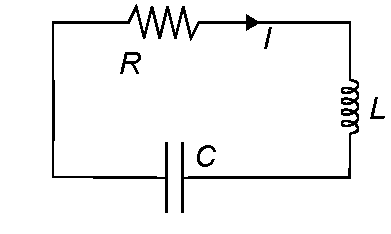
\includegraphics{RLC_circuit.pdf}
    \caption{LCR Circuit}
    \label{fig:LCR}
\end{figure}
By adding a resistor to an LC circuit we can add a form of damping. The voltage across the resistor is given by,
\begin{equation}
    V_R = RI = R\Dot{q}.
\end{equation}
So, the ODE becomes,
\begin{equation}
    L\Ddot{q} + R\Dot{q} + \frac{1}{C}q = 0.
\end{equation}
We can then conclude that the, for light damping, 
\begin{equation}
    q = q_0 \exp\left(\frac{R}{2L}t\right)\cos(\omega t)
\end{equation}
where,
\begin{equation}
    \omega^2 = \frac{1}{LC} - \frac{R^2}{4L^2},
\end{equation}
and
\begin{equation}
    Q = \frac{1}{R}\sqrt{\frac{L}{C}}.
\end{equation}
\section{General Damped Harmonic Oscillator}
Just as with SHM, we can describe a general equation of a damped harmonic oscillator,
\begin{equation}
    \alpha \Ddot{Z} + \kappa \Dot{Z} + \beta Z = 0 
\end{equation}
whose solution will be,
\begin{equation}
    Z(t) = Z_0 \exp\left(\frac{\kappa}{2\alpha}t\right)\cos\left(\sqrt{\frac{\beta}{\alpha}} + \phi\right).
\end{equation}
We introduced a new symbol,
\begin{definition}[$\kappa$]
    The constant representing the magnitude of the damping force.
\end{definition}
\chapter{Driven, Damped Harmonic Oscillator}
This is oscillatory motion where a driving force is provided. The driving force is given by,
\begin{equation}
    F(t) = F_0\cos(\omega t).
\end{equation}
We can then modify the equation of motion,
\begin{equation}
    \Ddot{x} + \gamma\Dot{x} + \omega_0^2 x = \frac{F_0}{m}\cos{\omega t},
\end{equation}
which we can rewrite in its exponential form,
\begin{equation} \label{forced}
    \Ddot{z} + \gamma\Dot{z} + \omega_0^2z = \frac{F_0}{m}e^{i\omega t}.
\end{equation}
NOTE: When we write functions in exponential form, we represent physical values with \textbf{only} the real part. We can then intuit an expression for $z$,
\begin{equation}
    z(t) = A(\omega)e^{(i\omega t  + \delta)}
\end{equation}
where $\delta$ is the phase between the actual oscillations and the driving force. Differentiating, substituting back into equation \eqref{forced}, and then dividing by $e^{(i\omega t + \delta)}$. The equation then has real and imaginary parts,
\begin{align}
    (\omega_0^2 - \omega^2)A(\omega) &= \frac{F_0}{m}\cos\delta & \Re, \\
    \gamma \omega A(\omega) &= \frac{F_0}{m}\sin\delta & \Im.
\end{align}
The phase is then given by,
\begin{equation}
    \tan \delta = \frac{\gamma \omega}{\omega_0^2 - \omega^2},
\end{equation}
and the amplitude function is given by,
\begin{equation}
    A(\omega) = \frac{F_0}{m\sqrt{(\omega_0^2 - \omega^2}^2 + (\omega\gamma)^2}.
\end{equation}
We must consider the limits of the function,
\begin{align}
    \omega &\to 0 & A(\omega) \to \frac{F_0}{m\omega_0^2} \\
    \omega &\to \infty & A(\omega) \to 0 \\
    \omega &\to \omega_0 & A(\omega) \to \frac{F_0}{m\omega_0\gamma} \\
    A_{\text{MAX}}&=\frac{F_0}{m\omega_0\gamma}\frac{1}{\sqrt{1-\left(\frac{\gamma}{2\omega_0}\right)^2}} & A_{\text{MAX}} \approx A(\omega_0) \to \text{Light damping}
\end{align}
\section{Transient Response}
The previous solution is what dominates. There is also the immediate transient response, which dies down pretty quickly. This will simply be the homogeneous solution to the equation, which is the solution to the damped harmonic oscillator.
\section{AC Circuit}
\begin{figure}[h]
    \centering
    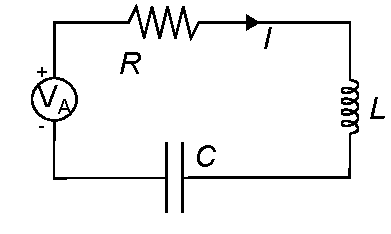
\includegraphics{RLC_driven.pdf}
    \caption{An LCR circuit with added AC.}
    \label{fig:AC}
\end{figure}
We can add a driving AC, with a voltage,
\begin{equation}
    V_A = V_0e^{i\omega t},
\end{equation}
which modifies the equation as so,
\begin{equation}
    L\Ddot{q} + R \Dot{q} + \frac{1}{C}q = V_0e^{i\omega t}
\end{equation}
whose solution is,
\begin{equation}
    q = A(\omega)e^{i(\omega t - \delta)}
\end{equation}
where
\begin{equation}
    A(\omega) = \frac{V_0}{\sqrt{(\omega_0^2-\omega^2)+ (\gamma\omega)^2}}
\end{equation}
and
\begin{align}
    \omega_0^2 &= \frac{1}{LC} & \gamma = \frac{R}{L}.
\end{align}
\subsection{Impedance}
The voltage and current in the resistor are in phase with the AC supply, however in the inductor and capacitor they are not. We can find the phase of the current by,
\begin{equation}
    I(t) = I_0e^{i\omega t},
\end{equation}
then the voltage is given by,
\begin{equation}
    V_L = L\dv{I}{t} = i\omega L I_0e^{i\omega t}
\end{equation}
which implies that $V_L$ leads $I$ by a phase of $\frac{\pi}{2}$. \\\\
We are able to do the same for the capacitance,
\begin{equation}
    \begin{split}
        V_C &= \frac{1}{C}q\\
        & = \frac{1}{C}\int I \dd{t} \\ 
        & = \frac{1}{i\omega C}I_0 e^{i\omega t} = -\frac{i}{\omega C}I.
    \end{split}
\end{equation}
Thus, $V_C$ lags $I$ by $\frac{\pi}{2}$.\\\\
We can represent this lead and lag through Ohm's law,
\begin{equation}
    V = IZ
\end{equation}
where $Z$ is the \textbf{impedance}. This is a complex function where the real part represents the \textbf{resistance} and the imaginary part represents the \textbf{reactance}.
\begin{equation}
    Z = R + i\left( \omega L - \frac{1}{\omega C} \right).
\end{equation}
\section{Absorbed power}
The power absorbed by a driven, damped oscillator is equal to the rate at which energy is dissipated. So,
\begin{equation}
    P = \frac{W}{\Delta t} = F_D v.
\end{equation}
We can then derive the instantaneous power,
\begin{equation}
    P(t) = b(v_0(\omega))^2\sin^2(\omega t - \delta).
\end{equation}
We can then get the average power absorbed per cycle by evaluating the integral, 
\begin{equation}
    \overline{P}(\omega) = \frac{1}{T}\int_{t_0}^{t_0 + T}b(v_0(\omega))^2\sin^2(\omega t - \delta),
\end{equation}
which gives,
\begin{equation}
    \overline{P}(\omega) = \frac{1}{2}b(v_0(\omega))^2 - \frac{\omega^2 F_0^2 \gamma^2}{2m\left[\left(\omega^2 -\omega_0^2\right)^2 + \omega^2\gamma^2\right]}.
\end{equation}
From this function, we can obtain a power-resonance curve.
\begin{center}
    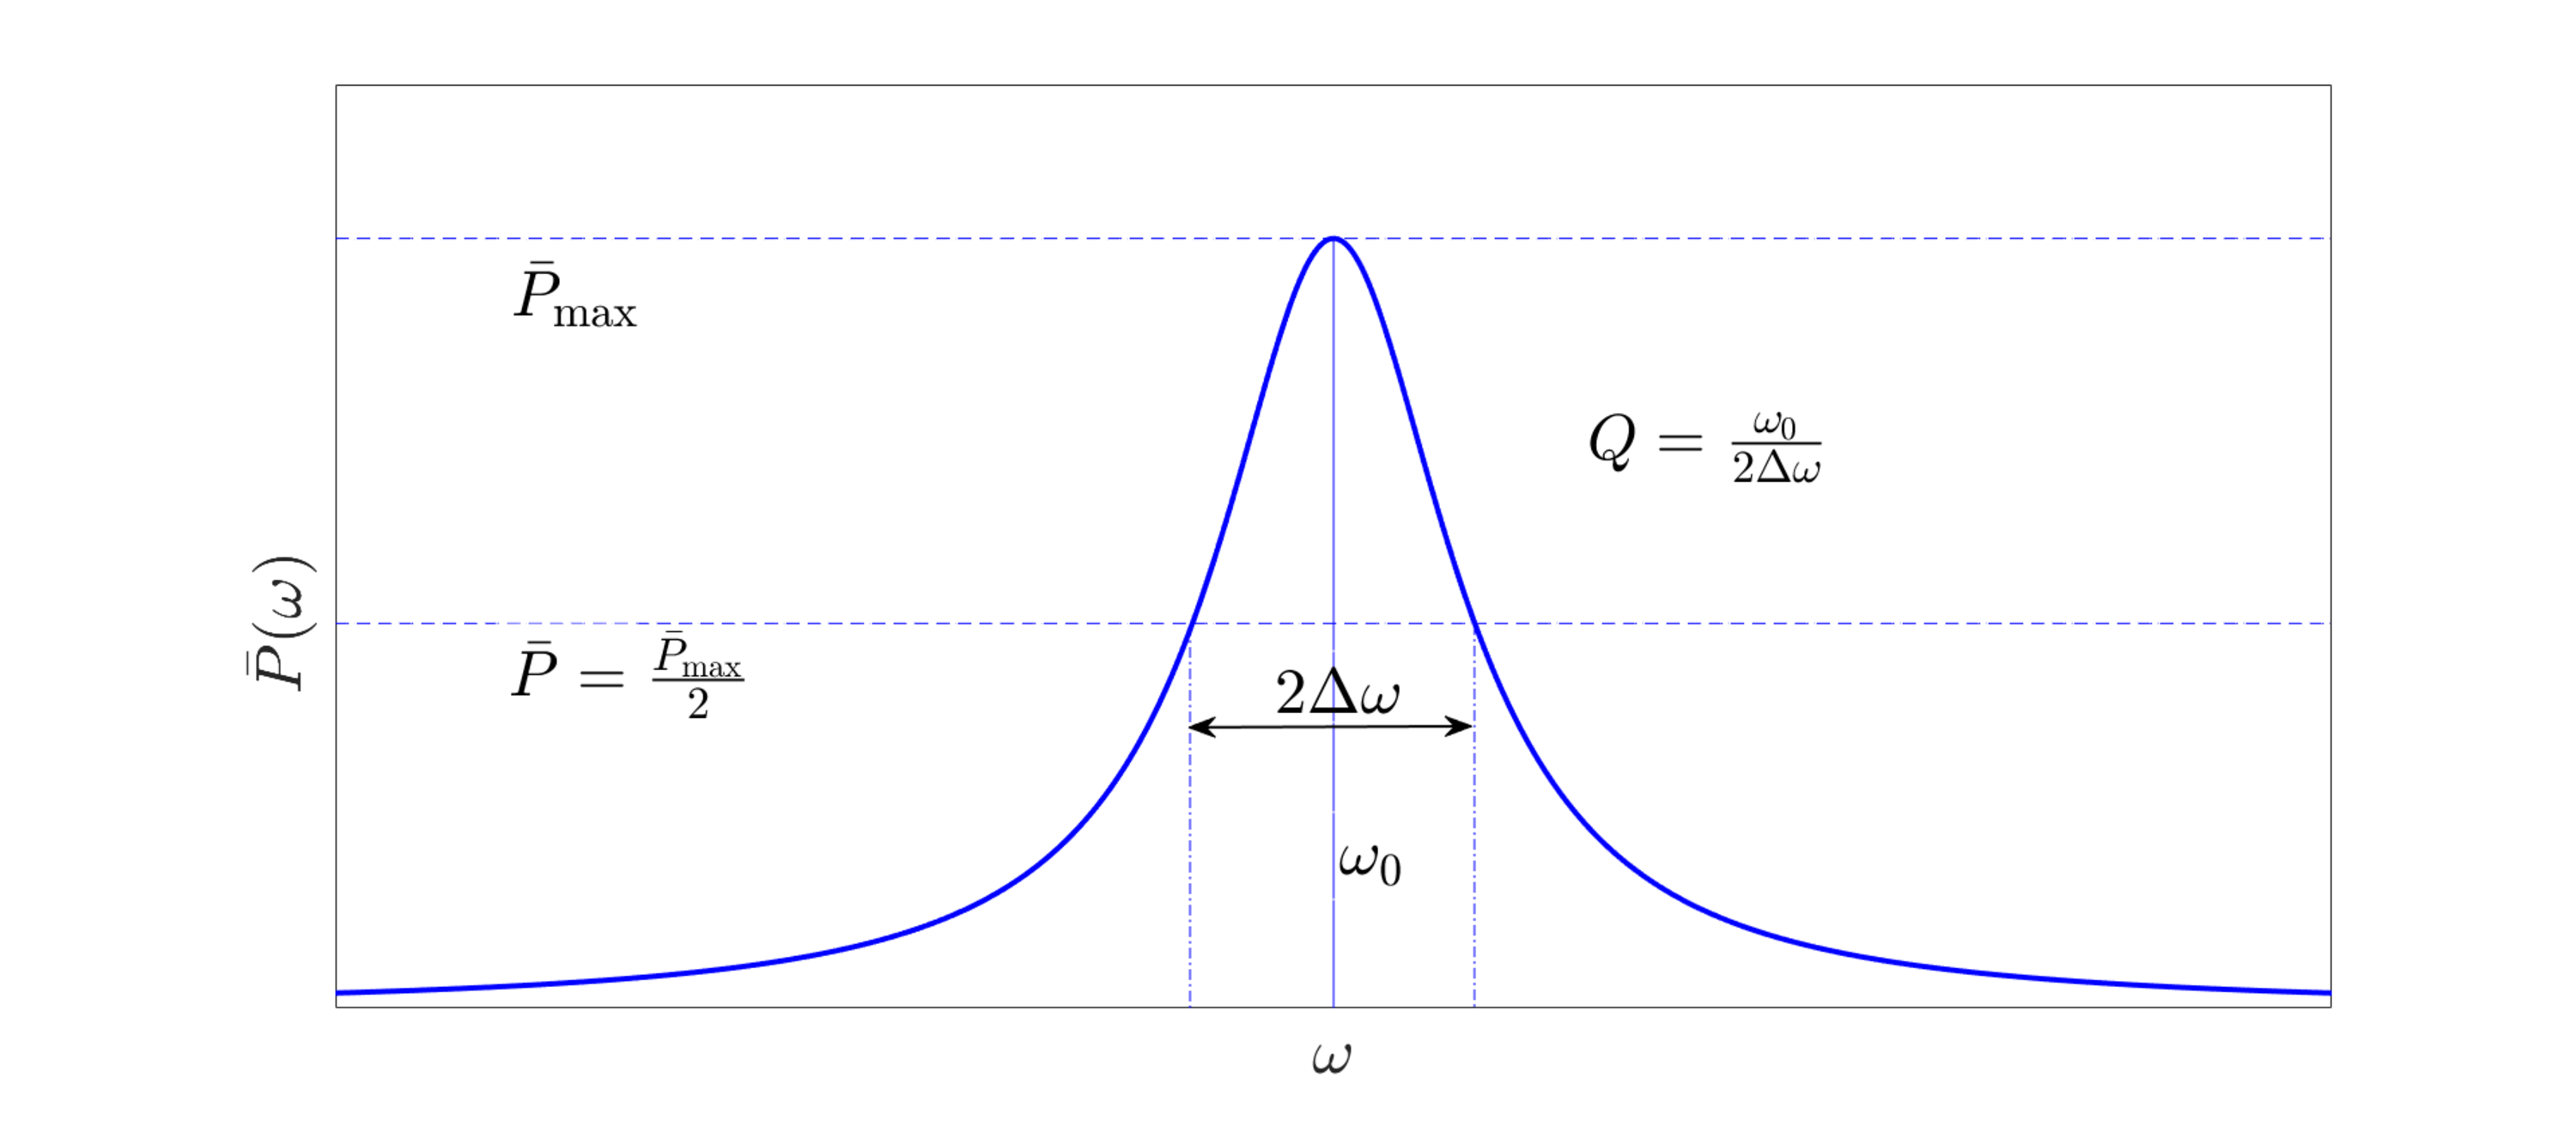
\includegraphics[width=\textwidth]{Power_resonance.pdf}
\end{center}
The width of the curve where $\omega = \omega_0$ defines the sharpness of the resonance. When close to the peak, we say $\omega \sim \omega_0$, so $\omega + \omega_0 \sim 2\omega_0$ and we can define $\Delta \omega = \omega - \omega_0$. Further,

\begin{equation}
    \omega_0^2 - \omega^2 = (\omega_0 + \omega)(\omega_0 - \omega) = 2\omega_0\Delta\omega.
\end{equation}
So, we can rewrite our power curve equation as,
\begin{equation}
    \overline{P}(\omega) = \frac{F_0^2}{2m\gamma\left(\frac{4\Delta \omega^2}{\gamma^2} + 1\right)}.
\end{equation}
The maximum value of power is then,
\begin{equation}
    \overline{P}_{\text{max}} = \frac{F_0^2}{2m\gamma}.
\end{equation}
We can define the full width at half height ($\omega_{\text{fwhh}}$) where $\overline{P}(\omega) = \frac{1}{2}\overline{P}_{\text{max}}$. Thus,
\begin{equation}
    \omega_{\text{fwhh}} = 2\Delta \omega = \gamma.
\end{equation}
This allows us to redefine the quality factor,
\begin{equation}
    Q = \frac{\omega_0}{\gamma} = \frac{\omega_0}{\omega_{\text{fwhh}}}.
\end{equation}
\chapter{Coupled Oscillators}
Coupled oscillators are joined together. We will first consider two identical pendula, $A$ and $B$ of mass $m$ and length $l$ coupled by a spring of spring constant $k$. We will consider two normal modes of oscillation (see figure \ref{fig:coupled}).
\begin{figure}[h]
    \centering
    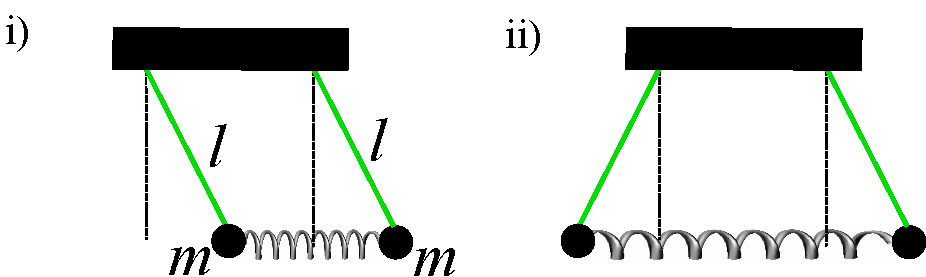
\includegraphics[width=200pt]{coupled_osc10.pdf}
    \caption{}
    \label{fig:coupled}
\end{figure}
\\
\begin{center}
\begin{tabular}{ c | V{4cm} | V{6cm} }
     & Description & Implications \\\hline
    i) & Each pendulum is displaced by the same amount in the same direction &  \begin{itemize}
        \item They will oscillate with the same frequency $\omega_1^2 = \frac{g}{l}$.
        \item They will be in phase.
    \end{itemize} \\ \hline
    ii) & Each pendulum is displaced by the same amount but in opposite directions. & \begin{itemize}
        \item They oscillate with the same frequency, $\omega_2$, which is different from $\omega_1$. 
        \item They will be out of phase.
    \end{itemize}
\end{tabular}
\end{center}

\begin{figure}[h]
    \centering
    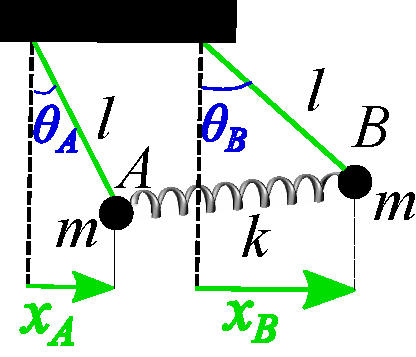
\includegraphics[width=100pt]{coupled_osc12.pdf}
    \caption{}
    \label{fig:cop}
\end{figure}
\section{Equations of motion in coupled pendula}
\noindent We will now consider the case where $x_B > x_A$ as in figure \ref{fig:cop}. The tension in the spring is given by,
\begin{equation}
    T = k(x_B - x_A)
\end{equation}
so the restoring force on B and A, using the small angle approximation, is given by,
\begin{align}
    F_B & = -\frac{mgx_B}{l}-k(x_B - x_A) & F_A = -\frac{mgx_A}{l} + k(x_B + x_A).
\end{align}
This gives the equations of motion,
\begin{align}
    \Ddot{x}_A + \frac{g}{l}x_A - \frac{k}{m}(x_B - x_A) & = 0 \label{A} \\
    \Ddot{x}_B + \frac{g}{l}x_B - \frac{k}{m}(x_B - x_A) & = 0. \label{B}
\end{align}
Now, let us define,
\begin{equation}
    q_n = \begin{cases}
        n = 1 & x_A + x_B \\
        n = 2 & x_A - x_B
    \end{cases} \label{normalcooord}
\end{equation}
which are the \textbf{normal coordinates} for our setup.
We can then perform \eqref{A} + \eqref{B} and \eqref{A} - \eqref{B} respectively,
\begin{align}
    \Ddot{q}_1 + \frac{g}{l} q_1 & = 0 \\
    \Ddot{q}_2 + \left(\frac{g}{l} + \frac{2k}{m}\right)q_2 & = 0,
\end{align}
where we can say,
\begin{equation}
    \omega_n^2 = \begin{cases}
        n = 1 & \dfrac{g}{l} \\
        n = 2 & \left(\dfrac{g}{l} + \dfrac{2k}{m}\right).
    \end{cases}
\end{equation}
As we can see, the normal coordinates are useful as they allow us to write decoupled versions of the equations of motion, representing the two normal modes of the motion of the pendulums. It can be viewed experimentally that when we excite a coupled system in a certain normal  mode, it will stay in that normal mode, or a combination of normal modes as it cannot transfer energy between them. Thus, we can solve and model \textit{any} motion of the coupled pendula by using a number of linear combinations of the normal mode equations.
\\\\
For the example presented here, the most general solutions take the form,
\begin{align}
	x_a &= C\cos(\omega_1 t - \delta_1) + D\cos(\omega_2 t - \delta_2)\\
	x_b &= C\cos(\omega_1 t - \delta_1) - D\cos(\omega_2 t - \delta_2)
\end{align} 
The sign change occurs because we know for the normal mode $\omega_1$, $x_a = x_b$, so the signs are the same. We change sign for the term representing the second normal mode $\omega_2$ as we have the condition $x_a = -x_b$. 
\subsection{Normal Modes for higher $n$}
We previously considered only the normal mode of a coupled oscillator by a single mass, $n=1$. Higher $n$ require Eigen analysis. 
\subsubsection{2 Masses - $n = 2$}
\begin{figure}
    \centering
    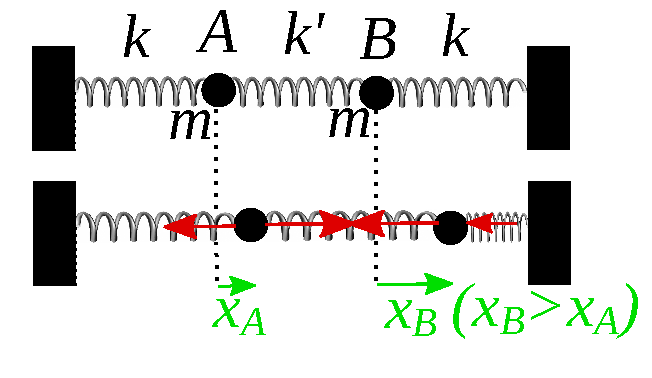
\includegraphics[width=150pt]{coupled_osc14.pdf}  
    \caption{Two masses connected by springs.}
    \label{fig:doublemass}
\end{figure}
We will be considering the setup in figure \ref{fig:doublemass}. We understand the governing equations are,
\begin{align}
    m\Ddot{x}_A & = -kx_A + k'(x_B - x_A)\label{eq1} \\
    m\Ddot{x}_B & = -kx_B - k'(x_B - x_A)\label{eq2}.
\end{align}
We will denote,
\begin{align*}
    \omega^2 & = \frac{k}{m} & \omega'^2 & = \frac{k'}{m},
\end{align*}
We then rewrite \eqref{eq1} and \eqref{eq2},
\begin{align}
    \Ddot{x}_A + \omega^2x_A + \omega'^2(x_A - x_B) & = 0 \label{eq3} \\
    \Ddot{x}_B + \omega^2x_B + \omega'^2(x_B - x_A) & = 0.\label{eq4}
\end{align}
We can assume that both of the masses will have the same frequency, $\Omega$. We can then assume trial equations,
\begin{align}
    x_A & = X_Ae^{i\Omega t}; & x_B & = X_Be^{i\Omega t}.\label{eq5}
\end{align}
Substituting \eqref{eq5} into \eqref{eq3} and \eqref{eq4}, and dividing by $e^{i\Omega t}$,
\begin{align}
    -\Omega^2X_A + \omega^2X_A + \omega'^2(X_A-X_B) = 0 \label{eq6} \\
    -\Omega^2X_B + \omega^2X_B + \omega'^2(X_B-X_A) = 0\label{eq7}.
\end{align}
Then, collecting like terms,
\begin{align}
    (\omega^2 + \omega'^2)X_A - \omega'^2X_B &= \Omega^2X_A \label{eq8} \\
    -\omega'^2X_A + (\omega^2 + \omega'^2)X_B &= \Omega^2X_B. \label{eq9}
\end{align}
We can rewrite this in vector form,
\begin{equation*}
    \begin{pmatrix}
        \omega^2 + \omega'^2 & -\omega'^2 \\
        -\omega'^2 & \omega^2 + \omega'^2
    \end{pmatrix}\begin{pmatrix}
        X_A \\ X_B
    \end{pmatrix} = \Omega^2 \begin{pmatrix}
        X_A \\ X_B
    \end{pmatrix}.
\end{equation*}
We will notice that this equation is in the form,
\begin{equation*}
    \vb{A}\vb{x} = \lambda\vb{x}
\end{equation*}
thus, we can perform Eigen analysis on this problem by solving the equation $|\vb{A} - \Omega^2\vb{I}|$,
\begin{equation*}
    \begin{split}
        (\omega^2 + \omega'^2 - \Omega^2)^2 - \omega'^4 & = 0 \\
        \omega^2 + \omega'^2 - \Omega^2 & = \pm\omega'^2. 
    \end{split}
\end{equation*}
Thus, we have two Eigen values,
\begin{align}
    \Omega^2 & = \omega^2  = \frac{k}{m} \label{eq10} \\
    \Omega^2 & = \omega^2 + 2\omega'^2 = \frac{k}{m} + \frac{2k'}{m} \label{eq11}.
\end{align}
We then have two normal modes for the system,
\begin{enumerate}
    \item By substituting \eqref{eq10} into \eqref{eq8},
    \begin{equation}
        X_A = X_B
    \end{equation}
    \item By substituting \eqref{eq11} into \eqref{eq8} or \eqref{eq9},
    \begin{equation}
        X_A = -X_B
    \end{equation}
\end{enumerate}
\subsubsection{Linear Triatomic Molecule $n = 3$}
\begin{figure}
    \centering
    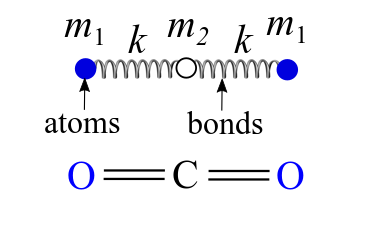
\includegraphics[width=150pt]{coupled_osc16.png}
    \caption{}
    \label{fig:n=3}
\end{figure}
Look at figure \ref{fig:n=3}. We can model this as a 3-mass problem moving in 1 dimension. We will define the factors,
\begin{align}
    \omega^2 = \frac{k}{m_1} && \omega'^2 = \frac{k}{m_2} && x_n(t) = x_ne^{i\Omega t}
\end{align}
for $n = \left\{1,2,3\right\}$. When we write down the governing equations, we are able to once again perform eigen analysis on the system,
\begin{equation}
    \begin{pmatrix}
        \omega^2 & -\omega^2 & 0 \\
        -\omega'^2 & 2\omega'^2 & -\omega'^2 \\
        0 & -\omega^2 & \omega^2
    \end{pmatrix}\begin{pmatrix}
        X_1 \\ X_2 \\ X_3
    \end{pmatrix} = \Omega^2 \begin{pmatrix}
        X_1 \\ x_2 \\ X_3
    \end{pmatrix}.
\end{equation}
Performing Eigen analysis, we obtain 3 Eigen values and 3 normal modes. 
\begin{enumerate}
    \item $\Omega^2 = 0$, transnational motion.
    \begin{align*}
        \omega^2X_1 - \omega^2X_2 = 0 & \implies X_1 = X_2 \\
        -\omega^2X_" + \omega^2X_3 = 0 & \implies X_2 
    \end{align*}
    \item $\Omega^2 = \omega^2$, symmetric stretching. 
    \begin{align}
        X_2 & = 0, & X_1 & = -X_3.
    \end{align}
    \item $\Omega^2 = 2\omega'^2 + \omega^2$
    \begin{equation*}
        X_3 = X_1 = -\frac{\omega^2}{2\omega'^2}X_2
    \end{equation*}
\end{enumerate}
\section{Transverse Oscillations}
These are oscillations which are displaced in the $y$ direction.
\subsection{Single Oscillator}
\begin{figure}
    \centering
    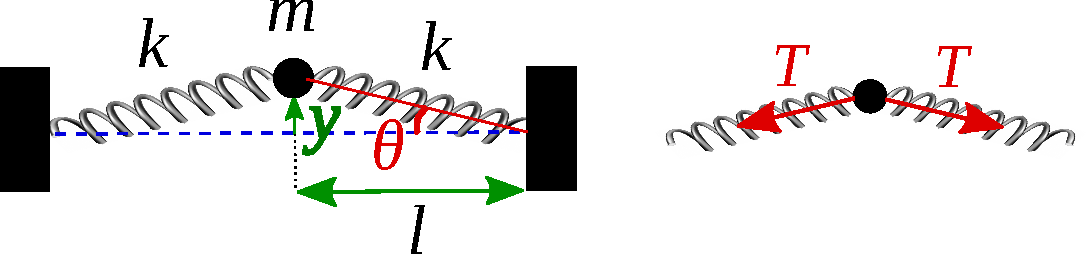
\includegraphics[width=200pt]{trasnverseosc.pdf}
    \caption{}
    \label{fig:trans}
\end{figure}
We are modelling a setup like that in figure \ref{trans}. We write this motion simply by asserting that $T$ remains constant.
\begin{proof}
    For a displacement $y$, each spring displaces by an amount $\Delta l$ such that,
    \begin{align*}
        (l +  \Delta l) \cos\theta = l 
    \end{align*}
    where
    \begin{align*}
        \theta = \arctan\left(\frac{y}{l}\right).
    \end{align*}
    We can write,
    \begin{equation*}
        \Delta l = l\left(\frac{1}{\cos\theta} - 1\right).
    \end{equation*}
    For small $\theta$, we can use the Taylor expansion of $\cos\theta$ to write $\Delta l$ as,
    \begin{equation}
        \Delta l = l \frac{\theta^2}{2}
    \end{equation}
    if $\theta$ is small. Thus, $\theta^2$ can be neglected, and the tension $T$ is constant.
\end{proof}
\noindent
Our equation of motion is then,
\begin{equation*}
    m \Ddot{y} = -2T\sin\theta
\end{equation*}
and
\begin{equation}
    \sin\theta \approx \tan\theta = \frac{y}{l}
\end{equation}
so, we can rewrite,
\begin{equation}
    \Ddot{y} = -\frac{2T}{ml}y
\end{equation}
which is an equation of SHM.
\subsection{2 Oscillators}
\begin{figure}
    \centering
    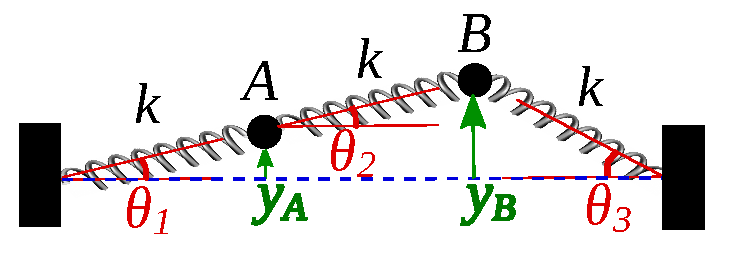
\includegraphics[width=250pt]{trasnverseosc2.pdf}
    \caption{}
    \label{fig:trans2}
\end{figure}
We are now modelling the setup in figure \ref{trans2}. Making the same assumptions as before, we can write the equations of motion,
\begin{align}
    m\Ddot{y}_A & = -T\sin\theta_1 + T\sin\theta_2 = \frac{T}{l}(y_B - 2y_A) \\
    m\Ddot{y}_B & = -T\sin\theta_2 - T\sin\theta_3 = \frac{T}{l}(y_A - 2y_B).
\end{align}
We can once again apply Eigen analysis and find the Eigen values to find the normal modes,
\begin{align}
    \Omega^2 & = \frac{T}{ml} & Y_A & = Y_B \\
    \Omega^2 & = \frac{3T}{ml} & Y_A & = -Y_B
\end{align}
\subsection{Higher $n$}
At higher $n$, the normal modes start being analogous to standing waves.
\section{Forced Coupled Oscillators}
\begin{figure}
    \centering
    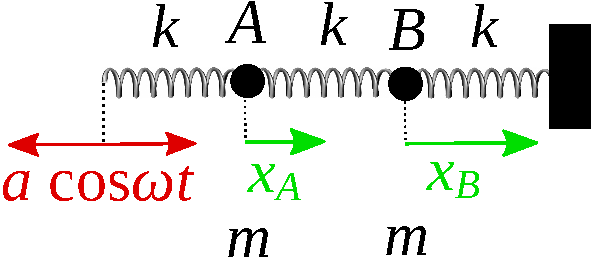
\includegraphics[width=200pt]{forcedcouple.pdf}
    \caption{}
    \label{fig:forcedcouple}
\end{figure}
Let us consider the setup as in figure \ref{fig:forcedcouple}. This is a 2 mass system, with $A$ being connected to a sinosudial drive with displacement $\epsilon = a\cos\omega t$. We have,
\begin{align}
    \Ddot{x}_A + \frac{2k}{m}x_A - \frac{k}{m}x_B & = \frac{F_0}{m}\cos\omega t \\
    \Ddot{x}_B - \frac{k}{m}x_A + \frac{2k}{m}x_B & = 0
\end{align}
where $F_0 = ka$. We can define the normal coordinates like we did in \eqref{normalcooord}. Our equations of motion then become, 
\begin{align}
    \Ddot{q}_1 + \frac{k}{m}q_1 & = \frac{F_0}{m}\cos\omega t \\
    \Ddot{q}_2 + \frac{3k}{m}q_2 & = \frac{F_0}{m}\cos\omega t
\end{align}
These are both equations of undamped, forced harmonic motion. We know then that the solutions are,
\begin{align}
    q_1 & = C_1(\omega)\cos(\omega t -\delta_1) & q_2 = C_2(\omega)\cos(\omega t - \delta_2)
\end{align}
where we define the following,
\begin{align}
    \omega^2_n & = \begin{dcases}
        \frac{k}{m} & n = 1 \\
        \frac{3k}{m} & n=2
    \end{dcases} \\
    \delta_n & = \begin{cases}
        0 & \omega < \omega_n \\
        \pi & \omega > \omega_n 
    \end{cases} \\
    C_n & = 
        \frac{F_0/m}{\omega_n^2 - \omega^2}
\end{align}
\chapter{Waves}
There are two types of waves, \textit{standing} and \textit{travelling} waves. \\\\
Travelling waves come in two forms,
\begin{enumerate}
    \item \textbf{Longitudinal} - Change in physical quantity is in direction of travel.
    \item \textbf{Transverse} - Change is orthogonal to direction of travel. 
\end{enumerate}
Further, these may either be,
\begin{enumerate}
    \item \textbf{Mechanical} - requires a medium.
    \item \textbf{Non-mechanical} - does not require a medium.
\end{enumerate}
\section{1D Wave Equation}
All waves are generated by a wave equation. For a distribution $y(x,t)$, the wave equation is given by,
\begin{equation}
    \pdv[2]{y}{t} = v^2\pdv[2]{y}{x},
\end{equation}
where $v$ is the velocity at which the wave propagates.
\subsection{Sinusoidal Waves}
Sinusoidal waves can be given by,
\begin{equation}
    y(x,t) = A\sin\left[\frac{2\pi}{\lambda}(x-vt)\right].
\end{equation}
A travelling sinusoidal wave will have frequency,
\begin{equation}
    \nu = \frac{v}{\lambda}.
\end{equation}
We can then define other properties of the wave,
\begin{align}
    \nu & = \frac{1}{T} & \omega & = 2\pi\nu.
\end{align}
We can define the wave number, $k = \frac{2\pi}{\lambda}$. We can then re-write the equation as,
\begin{equation}
    y(x,t) = A\sin(kx - \omega t)
\end{equation}
and we can rewrite the velocity of propagation as,
\begin{equation}
    v = \frac{\omega}{k}.
\end{equation}
\subsection{General solution to 1D wave equation}
The general solution takes the form,
\begin{equation}
    y(x,t) = f(x-vt) + g(x-vt)\label{eq:1dsol}.
\end{equation}
\begin{proof}
    Let us first define,
    \begin{equation}
        u = x - vt.
    \end{equation}
    We then differentiate $f$ with respect to $x$ and $t$.
    \begin{enumerate}
        \item \begin{equation}
            \pdv{f}{x} = \dv{f}{u}\pdv{u}{x}
        \end{equation}
        \item \begin{equation}
            \pdv[2]{f}{x} = \pdv{}{x}\left(\pdv{f}{u}\pdv{u}{x}\right) = \dv[2]{f}{u}\left(\pdv{u}{x}\right)^2 + \dv{f}{u}\pdv[2]{u}{x}
        \end{equation}
        \begin{align}
            \pdv{u}{x} = 1 && \pdv[2]{u}{x}=0\\
            &\pdv[2]{f}{x} = \dv[2]{f}{u}& \label{eq:2}
        \end{align}
        \item \begin{equation}
            \begin{split}
                \pdv{f}{t} = \dv{f}{u}\pdv{u}{t} & = -v\dv{f}{u} \\
                & \implies \pdv[2]{f}{t} = v^2 \dv[2]{f}{u} \label{eq:1}
            \end{split}
        \end{equation}
    \end{enumerate}
    Combining \eqref{eq:1} and \eqref{eq:2},
    \begin{equation}
        \pdv[2]{f}{t} = v^2\pdv[2]{f}{x}. \label{eq:3}
    \end{equation}
    We similarly get,
    \begin{equation}
        \pdv[2]{g}{t} = v^2\pdv[2]{g}{x}. \label{eq:4}
    \end{equation}
    Adding \eqref{eq:3} and \eqref{eq:4}, we get,
    \begin{equation}
        \pdv[2]{f+g}{t}= v^2\pdv[2]{f+g}{x},
    \end{equation}
    which is the same form as the 1D wave equation. So, \eqref{eq:1dsol} is a general solution of the 1D wave equation.
\end{proof}
\subsection{Velocity of travelling waves on a stretched string}
\begin{figure}[b]
    \centering
    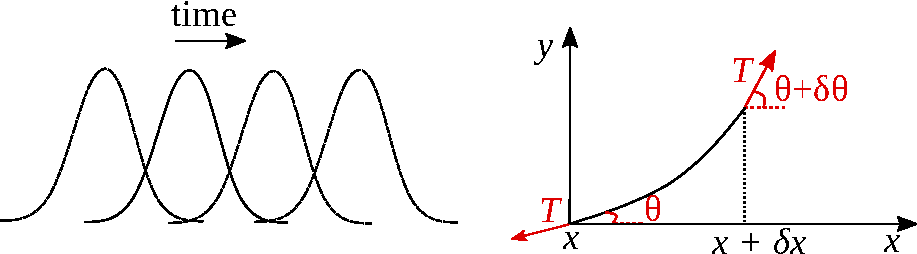
\includegraphics[width=300pt]{string.pdf}
    \caption{Stretched strings allow for waves to travel along their length.}
    \label{fig:stretchesstring}
\end{figure}
A string under tension $T$ and density $\mu$ can support transverse, travelling waves. We will consider a length of element of the string between $x$ and $\delta x$. We will consider that at $x$ the string is at an angle $\theta$ to the horizontal, and at an angle $\theta + \delta\theta$ at a distance $x + \delta x$. (See figure \ref{fig:stretchesstring}).
\\\\
The tension in the string at $x$,
\begin{equation}
\begin{split}
    & T\sin\theta \sim \theta \sim \tan\theta \approx \frac{\delta y}{\delta x} \implies \sin\theta = \pdv{x}{y} \\ &T\sin\theta = T\left(\pdv{y}{x}\right)_x.
\end{split}
\end{equation}
Similarly, tension at $x + \delta x$ is given by,
\begin{equation}
    T\sin(\theta + \delta\theta) \sim T\left(\pdv{y}{x}\right)_{x+\delta x}. \label{tensiondelta}
\end{equation}
We will now perform a first order Taylor expansion of \eqref{tensiondelta} about $x$,
\begin{equation}
    \begin{split}
        T\left(\pdv{y}{x}\right)_{x+\delta x} & = T\left\{\left(\pdv{y}{x}\right)_x + \pdv{}{x}\left(\pdv{y}{x}\right)_x\delta x\right\} \\
        & = T\left\{\left(\pdv{y}{x}\right)_x+\left(\pdv[2]{y}{x}\right)_x\right\}.
    \end{split}
\end{equation}
The net transverse force $F_y$ is the difference between the tensions at $x$ and $x + \delta x$,
\begin{equation}
    F_y = T\left\{\left(\pdv{y}{x}\right)_x + \left(\pdv[2]{y}{x}\right)_x\delta x - \left(\pdv{y}{x}\right)_x\right\} = T\pdv[2]{y}{x}\delta x.
\end{equation}
Similarly, for the $x$ component,
\begin{equation}
    F_x = T\cos(\theta + \delta\theta) - T\cos\theta \simeq T - T \simeq 0
\end{equation}
because,
\begin{equation}
    \cos(\theta + \delta \theta) \simeq \cos\theta \simeq 1 \text{ for small } \theta.
\end{equation}
We can apply a transverse disturbance to the string by accelerating it in the $y$ direction. By Newton's second law,
\begin{equation}
    \mu \delta x \pdv[2]{y}{t} = T\pdv[2]{y}{x}\delta x \implies \pdv[2]{y}{t} = \frac{T}{\mu}\pdv[2]{y}{x}
\end{equation}
which is the 1D wave equation for a wave with velocity
\begin{equation}
    v = \sqrt{\dfrac{T}{\mu}}. \label{velocitystring}
\end{equation}
\subsection{Energy Stored in a Wave}
Let us consider a string under tension. Let us consider a horizontal element $\delta x$ which has mass $\mu\delta x$ which oscillates in the $y$ direction. Its kinetic energy is given by,
\begin{equation}
    \delta K = \frac{1}{2}(\mu\delta x)\left(\pdv{y}{t}\right)^2. \label{kineticwave}
\end{equation}
Further, when not at equilibrium, the string is stretched so that it has an elemental, stretched length $\delta s$ under a tension $T$. It's potential energy can be then given by,
\begin{equation}
    \delta U = (\delta s - \delta x)T. \label{potentialwave}
\end{equation}
We understand,
\begin{equation}
    \delta s = \left(\delta x^2 + \delta y^2\right)^{\frac{1}{2}}\approx \delta x\left(1 + \frac{1}{2}\left(\pdv{y}{x}\right)^2\right),
\end{equation}
by binomial expansion, valid for small displacements. Then,
\begin{equation}
    \delta s - \delta x = \frac{1}{2}\left(\pdv{y}{x}\right)\delta x. 
\end{equation}
Thus, we can write the total energy element,
\begin{equation}
    \delta E = \delta U + \delta K = \frac{1}{2}\mu \delta x\left(\pdv{y}{t}\right)^2 \frac{1}{2}\left(\pdv{y}{x}\right)^2T.
\end{equation}
By \eqref{velocitystring},
\begin{equation}
    \delta E = \frac{1}{2}\mu\delta x\left[\left(\pdv{y}{t}\right)+ v^2\left(\pdv{y}{x}\right)^2\right],
\end{equation}
which we can integrate,
\begin{equation}
    E = \frac{1}{2}\int_a^b \mu\left[\left(\pdv{y}{t}\right)+ v^2\left(\pdv{y}{x}\right)^2\right]\dd{x}
\end{equation}
to find the energy stored in the string between $x=a \to x=b$.
\subsubsection{Power of a sinusoidal wave}
Let us consider a solution to the 1D wave equation $y = A\sin(kx -\omega t)$. By substituting this into \eqref{potentialwave} and \eqref{kineticwave} and integrating from $0 \to \lambda$, we can obtain the kinetic and potential energy over 1 wavelength,
\begin{align}
    K_{\lambda} = \frac{1}{4}\mu\omega^2A^2\lambda && U_{\lambda} = \frac{1}{4}\mu\omega^2A^2\lambda,
\end{align}
and adding these yields,
\begin{equation}
    E_{\lambda} = \frac{1}{2}\mu\omega^2A^2\lambda.
\end{equation}
The power is then $E_{\lambda}\times\frac{v}{\lambda}$, and thus,
\begin{equation}
    P = \frac{1}{2}\mu\omega^2A^2v.
\end{equation}
\section{Waves at Boundaries}
\begin{figure}
    \centering
    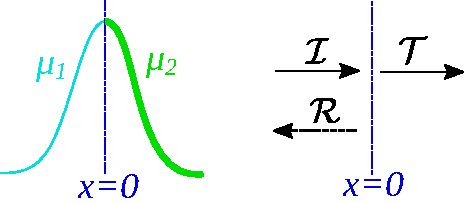
\includegraphics{reflected.pdf}
    \caption{}
    \label{fig:reflected}
\end{figure} \noindent
When waves encounter discontinuity, some fraction of the wave will be reflected back to us. At this discontinuity, there will be a \textit{incident}, \textit{reflected}, and \textit{transmitted} wave at the discontinuity.\\\\
To illustrate this, consider figure \ref{fig:reflected}, where the density of a string changes from $\mu_1$ to $\mu_2$ at the boundary $x=0$. The incident wave is described by,
\begin{equation}
    y_{\mathcal{I}} = \mathcal{I}\cos(k_1x - \omega t)
\end{equation}
the reflected wave is described by,
\begin{equation}
    y_{\mathcal{R}} = \mathcal{R}\cos(k_2x + \omega t)\end{equation}
and the transmitted wave is given by,
\begin{equation}
    y_{\mathcal{T}} = \mathcal{T}\cos(k_2x - \omega't).
\end{equation}
At the boundary, $\mu$ changes, and thus $v$ must also change. \textbf{However}, the string is continuous so the frequency of the exciting pulse must be equal in both regions $\omega = \omega'$, thus, $k$, and, equivalently, $\lambda$ must change. We understand $\omega = vk$, so,
\begin{equation}
    \omega = v_1k_1 = \omega' = v_2k_2
\end{equation}
hence,
\begin{equation}
    \frac{k_2}{k_1} = \frac{v_1}{v_2} = \sqrt{\frac{\mu_2}{\mu_1}} =\frac{\lambda_1}{\lambda_2} = n
\end{equation}
where $n$ is known as the \textit{refractive index}.
\\\\
We can further state that $\pdv{y}{x}$ is continuous across the boundary, because the restoring force is continuous across the boundary and the tension $T$ is constant. We can apply the continuity of this gradient as well as the continuity of $y$ in order to better describe the waves,
\begin{equation}
    y_{\mathcal{I}} + y_{\mathcal{R}} = y_{\mathcal{T}}
\end{equation}
which, when substituting and evaluating at $x = 0$, yields the first condition,
\begin{equation}
    \mathcal{I} + \mathcal{R} = \mathcal{T}.
\end{equation}
We can obtain the second condition by evaluating $\pdv{y}{x}$ at $x= 0$, 
\begin{equation}
    -k_1\mathcal{I} +k_1\mathcal{R} = -k_2\mathcal{T}.
\end{equation}
Using these we are able to express the reflected and transmitted amplitudes as a function of incident amplitude,
\begin{align}
    \frac{\mathcal{T}}{\mathcal{I}} = \frac{2k_1}{k_1 + k_2} = \frac{2}{n+1} = \frac{2\sqrt{\mu_1}}{\sqrt{\mu_1} +\sqrt{\mu_2}} & = \mathcal{T}_c & &\text{Transmission Coefficient}\\
    \frac{\mathcal{R}}{\mathcal{I}} = \frac{k_1 - k_2}{k_1 + k_2} = \frac{1-n}{1+n} & = \mathcal{R}_c & &\text{Reflection Coefficient}
\end{align}
Below are listed some properties of the coefficients,
\begin{enumerate}
    \item $0 < \mathcal{T}_c < 2 \implies$ Transmitted wave is always in phase with the incident wave
    \item $-1 < \mathcal{R}_c < 1$ and $\mathcal{R}_c < 0 \iff k_2 > k_1 \implies$ The reflected wave is only in phase with the incident wave if $n < 1$.
    \item If $k_1 \sim k_2$, $\mathcal{R}_c$ is small, $\implies$ there is hardly any relfection.
    \item When $k_2 \to \infty$, $\mathcal{T}_c \to 0$, and $\mathcal{R}_c\to-1 \implies$ no transmission occurs, we get total reflection, which results in \textit{standing waves}.
    \item $\mathcal{T}_c = 1 + \mathcal{R}_c$.
\end{enumerate}

\section{Standing Waves}
Before we talk about standing waves, we must understand the \textbf{principle of superposition}. It states that if $y_1(x,t)$ and $y_2(x,t)$ are both solutions to the wave equation, the linear combination,
\begin{equation}
	y(x,y) = A_1y_1(x,t) + A_2y_2(x,t)
\end{equation}
is also a solution. This follows from the fact that the wave equation is linear. 
\begin{proof}
	Consider the wave equation for $y_1$ and $y_2$. Multiply each by $A_1$ and $A_2$ respectively and add them together,
	\begin{equation}
		\begin{split}
			& A_1\pdv[2]{y_1}{t} + A_2\pdv[2]{y_2}{t} = v^2A_1\pdv[2]{A_1}{x} = v^2A_2\pdv[2]{y_2}{x} \\	
			\implies & \pdv[2]{}{t}\left(A_1y_1 + A_2y_2\right) = v^2\pdv[2]{}{t}\left(A_1y_1 + A_2y_2\right)
		\end{split}
	\end{equation}
	thus $A_1y_1 + A_2y_2$ is also a solution to the wave equation.
\end{proof}
Considering standing waves, let us imagine holding a string at a fixed length from $x=0$ to $x=L$. We have boundary conditions such that $\mathcal{T}_c = 0$ and $\mathcal{R}_c = -1$. The wave can be described the superposition of two waves of the same frequency and amplitude travelling in opposite directions. Then,
\begin{equation}
	\begin{split}
		y = y_{\mathcal{I}} + y_{\mathcal{I}} & = Ie^{i(\omega t - kx)} - Ie^{i(\omega t + kx)} \\
		& = Ie^{i\omega t}\left(e^{-ikx} - e^{ikx}\right) \\
		& = f(t)g(x).
	\end{split}
\end{equation}
Thus, we have seperated the wave into its time and spatial components. Given a fixed $x$, all points vivrate at the same frequency, but the spatial patterns vary along the string. \\\\
\textbf{EXAMPLE:} Consider the incident wave as, $y_{\mathcal{I}}(x,t) = \frac{A}{2}\sin(kx - \omega t)$. The superposition of the incident and reflected waves gives,
\begin{equation}
	y = y_{\mathcal{I}} + y_{\mathcal{R}} = \frac{A}{2}\sin(kx - \omega t) + \frac{A}{2}\sin(kx + \omega t).
\end{equation}
Using the trigonometric identity,
\begin{equation}
	\sin(\alpha + \beta) + \sin(\alpha - \beta) = 2\sin\alpha\cos\beta 
\end{equation}
we get,
\begin{equation}
	y = A\sin kx \cos\omega t.
\end{equation}
\subsection{Discrete normal modes}
Given that the string is fixed, $y$ must satisfy the boundary conditions, 
\begin{align}
	y(0, t) = 0 && \implies && \sin(k\cdot 0) = 0 \label{0cond} \\
	y(L,t) = 0 && \implies && \sin(kL) = 0 \label{lengthconditon}
\end{align}
In order for this to be possible, the values of $k$ must be restricted to,
\begin{equation}
	k_n = \frac{n\pi}{L}, n \in \mathbb{Z}.
\end{equation}
So, we have a \textit{discrete set of normal modes of oscillation}, such that, 
\begin{equation}
	y_n = A_n\sin\left(\frac{n\pi}{L}\right)\cos(\omega_nt)
\end{equation}
where 
\begin{equation}
	\omega_n = v k_n = \frac{vn\pi}{L}
\end{equation}
which is the angular frequency of the $n^{\text{th}}$ mode and $A_n$ is the amplitude of the $n^{\text{th}}$ mode.
\subsubsection{Wavelength of standing waves}
We have,
\begin{equation}
	k_n = \frac{2\pi}{\lambda_n} = \frac{n\pi}{L}
\end{equation}
so,
\begin{align}
	\lambda_n = \frac{2L}{n} && \implies && L = n\frac{\lambda_n}{2}
\end{align}
thus, a standing wave is obtained if an integer number of half-wavelengths fit onto a string. The frequency of teh standing wave is given by,
\begin{equation}
	\nu = \frac{n}{2L}\sqrt{\frac{T}{\mu}}.
\end{equation}
\subsubsection{Superposition of normal modes}
Most of the time, motion on a string will be given by the superposition of normal modes given by,
\begin{equation}
	\sum_n A_n\sin\left(\frac{n\pi x}{L}\right)\cos(\omega_n t).
\end{equation}
\section{Sound Waves}
Sound waves are longitudonal, which means that the direction of motion is the same as the direction of propogation. This means that their wave equation is given by,
\begin{equation}
	\pdv[2]{f}{t} = \frac{\gamma P_0}{\rho}\pdv[2]{f}{x}
\end{equation}
where $P_0$ is the equillibrium pressure, $\rho$ is the density, and $\gamma$ is the adiabatic index. The velocity of sound waves is then,
\begin{equation}
	v = \sqrt{\frac{\gamma P_0}{\rho}}.
\end{equation}

\section{The wave equation in 2 dimensions}
The wave equation on a membrane can be given by,
\begin{equation}
	\grad^2 f = \frac{\sigma}{T} \pdv[2]{f}{t}.
\end{equation}
where $f(x,y,t)$ is the displacement and T is the tension. Expanding this, the equation we wish to solve is,
\begin{equation}
	\left(\pdv[2]{}{x} + \pdv[2]{}{y}\right)f(x,y,t) = v^{-2}\pdv[2]{f(x,y,t)}{t}.
\end{equation}
We will now assume a solution,
\begin{equation}
	f(x,y,t) = f_x(x)f_y(y)f_t(t).
\end{equation}
Substituing this in, we get, 
\begin{equation}
	\begin{split}
		& \left(\pdv[2]{}{x} + \pdv[2]{}{y}\right)\left(f_x(x)f_y(y)f_t(t)\right) = v^{-2}\pdv[2]{f_x(x)f_y(y)f_t(t)}{t} \\
		\implies & f_y(y)f_t(t)\dv[2]{f_x(x)}{x} + f_x(x)f_t(t)\dv[2]{f_y(y)}{y} = v^{-2}f_x(x)f_y(y)\dv[2]{f_t(t)}{t}.
	\end{split}
\end{equation}
We can then divide through by $f_x(x)f_y(y)f_t(t)$, where we will find that each side only depends on its own variables, so we can equate the expression to a constant,
\begin{equation}
	\frac{1}{f_x(x)}\dv[2]{f_x(x)}{x} + \frac{1}{f_y(y)}\dv[2]{f_y(y)}{y} = v^{-2}\frac{1}{f_t(t)}\dv[2]{f_t(t)}{t} = -k^2.
\end{equation}
We can further seperate the $x$ and $y$ components,
\begin{equation}
	\frac{1}{f_x(x)}\dv[2]{f_x(x)}{x} = -k^2 - \frac{1}{f_y(y)}\dv[2]{f_y(y)}{y} = k_x^2,
\end{equation}
where equation for $f_y$ becomes,
\begin{equation}
	 \frac{1}{f_y(y)}\dv[2]{f_y(y)}{y} = -k_y^2
\end{equation}
so we have the relation,
\begin{equation}
	k^2 = k_x^2 + k_y^2.
\end{equation}
Thus, our probelm turns into 3 ordinary, second ordertial equations,
\begin{align}
	\dv[2]{f_x(x)}{x} & = -k_x^2f_x(x) \\	
	\dv[2]{f_y(y)}{y} & = -k_y^2f_y(y) \\
	\frac{1}{v^2} \pdv[2]{f_t(t)}{t} & = -k^2f_t(t).
\end{align}
For which the solutions are,
\begin{align}
	f_x(x) & = A_x\cos k_xx + B_x\sin k_x x \\
	f_y(y) & = A_y\cos k_yy + B_y\sin k_y y \\
	f_t(t) & = A_t\cos\omega t + B_t \cos\omega t
\end{align}
where $\omega^2 = k^2v^2$. The complete solution then takes the form,
\begin{equation}
	f(x,y,t) = f_x(x)f_y(y)f_t(t).
\end{equation}
\subsection{Solutions in exponential form}
\begin{align}
	f_x(x) &= c_xe^{\pm ik_x x} \\
	f_y(y) &= c_ye^{\pm ik_y y} \\
	f_t(t) &= c_te^{\pm i\omega t}
\end{align}
where the full solution becomes,
\begin{equation}
	f(x,y,t) = Ce^{i(k_xx + k_yy - \omega t)} = Ce^{i(\vb{k}\cdot\vb{x}-\omega t)}
\end{equation}
where,
\begin{align}
	\vb{k} = (k_x, k_y) && \vb{x} = (x,y).
\end{align}

\chapter{Dispersion and Interference}

\appendix
\chapter{Common Waveforms and Examples}
\section{Gaussian Pulse}
\begin{equation}
    y(x,t) = A\exp\left(-\frac{1}{a}(x-vt)^2\right)
\end{equation}

\section{Waves on a square membrane}
\section{Waves on a circular membrane}


\end{document}
